
%% A sample appendix
%%
%%**********************************************************************
%% Legal Notice:
%% This code is offered as-is without any warranty either
%% expressed or implied; without even the implied warranty of
%% MERCHANTABILITY or FITNESS FOR A PARTICULAR PURPOSE!
%% User assumes all risk.
%% In no event shall any contributor to this code be liable for any damages
%% or losses, including, but not limited to, incidental, consequential, or
%% any other damages, resulting from the use or misuse of any information
%% contained here.
%%**********************************************************************
%%
%% $Id: Appendix.tex,v 1.5 2006/08/24 21:12:47 Owner Exp $
%%

% N.B.: an appendix chapter starts with "appchapter" instead of "chapter"
%
% The first argument in [ ] is the title as displayed in the table of contents
% The second argument is the title as displayed here.  Use \\ as appropriate in
%   this title to get desired line breaks

%----------------------------------------------------------------------------------------
%	HLL fluxes
%----------------------------------------------------------------------------------------
\appchapter[Derivation of HLL fluxes]{Derivation of HLL fluxes}
\label{app:hll_flux}

The integral average over the Riemann fan: $[x_l,x_r] \times [0,t]$ if found with the conservation law
\begin{gather}
\label{eqn:hll_flux_1}
\int_{x_l}^{x_r} \mbf{U}(x,t) dx - \int_{x_l}^{x_r} \mbf{U}(x,0) dx + \int_{0}^{t} \mbf{F}(\mbf{U}(x_r,t')) dt'
- \int_{0}^{t} \mbf{F}(\mbf{U}(x_l,t')) dt' = 0.
\end{gather}
Integrating and subtracting the last terms of equation \eqref{eqn:hll_flux_1} gives
\begin{gather}
\label{eqn:hll_flux_2}
\int_{x_l}^{x_r} \mbf{U}(x,t) dx = x_r\mbf{U}_r - x_l\mbf{U}_l + t(\mbf{F}_l - \mbf{F}_r).
\end{gather}
Substituting $x_l  = t S_l$, $x_r  = t S_r$, into \eqref{eqn:hll_flux_2} and dividing it by $t(S_r - S_l)$, gives the integral average 
\begin{gather}
\label{eqn:hll_flux_3}
\frac{1}{t(S_r - S_l)}\int_{x_l}^{x_r} \mbf{U}(x,t) dx = \frac{S_r\mbf{U}_r - S_l\mbf{U}_l + \mbf{F}_l - \mbf{F}_r}{S_r - S_l}.
\end{gather}
The HLL intermediate state, $\mbf{U}^*$, is defined as the intergral average given above in \eqref{eqn:hll_flux_3}.

The HLL fluxes are found by integrating over the left or right half of the Riemann fan.  Integration over the right half, $[0,x_r] \times [0,t]$, and dividing by $t$, gives 
\begin{gather}
\label{eqn:hll_flux_4}
\frac{1}{t}\int_{0}^{x_r} \mbf{U}(x,t) dx = S_r\mbf{U}_r + \mbf{F}_r - \mbf{F}^*.
\end{gather}
Rearranging \eqref{eqn:hll_flux_4}, and approximating the integral of the left hand side with \eqref{eqn:hll_flux_4}, gives
\begin{gather}
\label{eqn:hll_flux_5}
\mbf{F}^* = \frac{S_r \mbf{F}_l - S_l \mbf{F}_r + S_r S_l (\mbf{U}_l - \mbf{U}_r) }{S_r - S_l}.
\end{gather}.

\clearpage

%----------------------------------------------------------------------------------------
%	Additional functionality
%----------------------------------------------------------------------------------------
%% \appchapter[Thrust: \verb+transorm_n+]{Thrust: \verb+transorm_n+}
\appchapter[Thrust templates]{Thrust templates}
\label{app:thrust_add}

Below are \verb+transform_n+ templates for unary and binary functors, as well as the inline function \verb+make_device_counting_iterator+ [A. Corrigan, private correspondence].  The type \verb+Struct+ is being iterated over when used in conjunction with \verb+make_device_counting_iterator+.
\begin{lstlisting}
namespace thrust
{
  template<typename InputIterator,
           typename Size,
           typename OutputIterator,
           typename UnaryFunction>
  OutputIterator transform_n(InputIterator first, Size n,
			     OutputIterator result,
			     UnaryFunction op)
	 {
	   return transform(first, first+n, result, op);
	 }
  template<typename InputIterator1,
           typename Size,
           typename InputIterator2,
           typename OutputIterator,
           typename BinaryFunction>
    OutputIterator transform_n(InputIterator1 first1, Size n,
			       InputIterator2 first2,
			       OutputIterator result,
			       BinaryFunction op)
	   {
	     return transform(first1, first1+n, first2, result, op);
	   }

} //end namespace

typedef int Index;
typedef thrust::device_vector<Struct>::iterator StructIterator;
typedef thrust::iterator_system<StructIterator>::type device_iterator_system;
typedef thr::counting_iterator<Index,device_iterator_system> device_counting_iterator;

inline device_counting_iterator make_device_counting_iterator(Index start=Index(0)) { return device_counting_iterator(start); }

\end{lstlisting}

\clearpage

%----------------------------------------------------------------------------------------
%	Kelvin-Helmholtz instability initial conditions
%----------------------------------------------------------------------------------------
\appchapter[Kelvin-Helmholtz instability initial conditions]{Kelvin-Helmholtz instability initial conditions}
\label{app:kh_instability_ics}

\begin{figure}[htbp]\figSpace
\begin{center} 
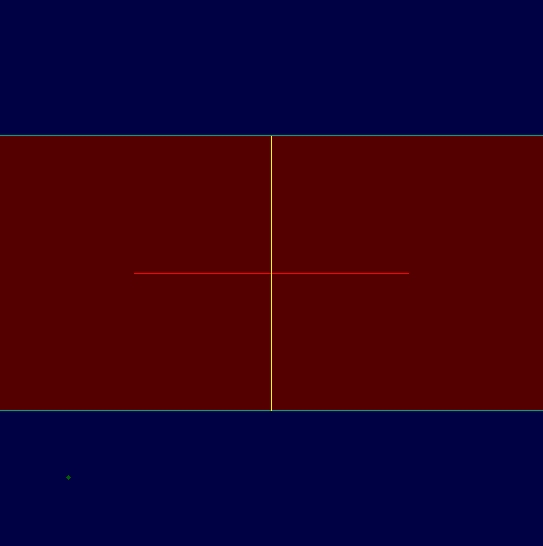
\includegraphics[width=0.5\textheight]{fig/kh0.jpg}
\caption{Initial conditions of the Kelvin-Helmoltz instability problem.  See Section~\ref{sec:gpu_results} for solutions at times t=1 and t=5.}
\end{center} 
\label{fig:kh_instability_ics}
\figSpace
\end{figure}


